\runningheader{SAT Mathematics}{Drill Set 10}{Page \thepage\ of \numpages}

\begingradingrange{sat-drill-10}
\subsection*{SAT Drill 10}

\question[1]
Given that $2(x+4)=18$, what is the value of $x+6$?
\begin{choices}
  \choice $-4$
  \choice $5$
  \CorrectChoice $9$
  \choice $11$
\end{choices}

\question[1]
Which of the following values is a solution to the given inequality?
\[
  3x+2<-5(x+6)
\]
\begin{choices}
  \choice $-5$
  \CorrectChoice $-4$
  \choice $3$
  \choice $4$
\end{choices}

\question[1]
The bar graph shows how many hours the air conditioner was on from Monday to Friday in a given week. What is the mean number of hours the air conditioner was on during this period?
\begin{center}
  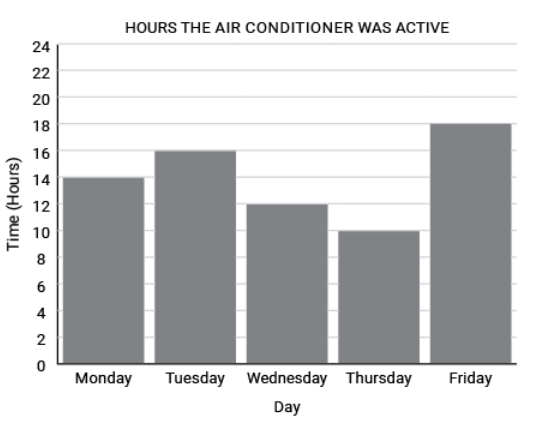
\includegraphics[width=0.90\linewidth]{images/cus18}
\end{center}
\begin{choices}
  \choice $8$
  \choice $10$
  \choice $12$
  \choice $14$
\end{choices}



\newpage




\question[1]
The expression $-2(x+3)^2+6$ is equivalent to $a x^2+b x+c$, where $a<0$ and $b<0$. What is the value of $c$?
\begin{solution}
-12
\end{solution}

\question[1]
What is the value of the slope of a line perpendicular to the line $5x-6y+30=0$?
\begin{solution}
$-\frac{6}{5}$
\end{solution}

\question[1]
If $m$ and $n$ are solutions to the given equation, what is the value of $m+n$?
\[
  3x^2+9x-27=0
\]
\begin{solution}
-3
\end{solution}

\question[1]
The graph of $(x-3)^2+y^2+8y=84$ is a circle in the $xy$-plane. Which of the following coordinates lie on the circle?
\begin{choices}
  \choice $(1,7)$
  \choice $(-2,5)$
  \CorrectChoice $(-3,4)$
  \choice $(3,-6)$
\end{choices}


\newpage


\question[1]
At the start of the winter, the US stockpile of corn was 5 billion bushels. Two months later, $p\%$ of the stockpile had been used. Which expression best represents the number, in billions, of bushels of corn remaining in the US stockpile at the end of those two months?
\begin{choices}
  \choice $2(5)\left(\frac{100-p}{100}\right)$
  \CorrectChoice $5\left(\frac{100-p}{100}\right)$
  \choice $\left(\frac{p}{100}\right)$
  \choice $2(5)(100-p)$
\end{choices}

\question[1]
The equation $P(y)=37(1.1)^y$ gives the estimated annual profit, in thousands of dollars, at a pottery studio, where $y$ is the number of years since the studio moved to a new location. Which of the following is the best interpretation of the number 37 in this context?
\begin{choices}
  \CorrectChoice The estimated annual profit, in thousands of dollars, when the studio moved to the new location
  \choice The increase in the estimated annual profit, in thousands of dollars, each year
  \choice The number of years since the studio moved to the new location
  \choice The percent increase in the estimated annual profit each year
\end{choices}

\question[1]
Triangle $JKL$ is an isosceles triangle. The measure of angle $J$ is $30^\circ$. If $JL$ is the longest side of the triangle, what is the measure of angle $K$?
\begin{choices}
  \choice $30$
  \choice $75$
  \CorrectChoice $120$
  \choice $150$
\end{choices}




\newpage




\question[1]
If $f(2x)=9x-7$, what is the value of $f(6)$?
\begin{choices}
  \choice $11$
  \CorrectChoice $20$
  \choice $47$
  \choice $101$
\end{choices}

\question[1]
How many solutions does the given system of equations have?
\[
  \begin{gathered}
  3x-4y=16 \\
  -6x=-8y+32
  \end{gathered}
\]
\begin{choices}
  \choice Exactly one
  \choice Exactly two
  \choice Infinitely many
  \CorrectChoice Zero
\end{choices}

\question[1]
If $\frac{5}{x}=\frac{2}{y}$ and $\frac{4}{x}-\frac{2}{y}=-\frac{1}{5}$, what is the value of $xy$?
\begin{solution}
10
\end{solution}

\question[1]
In the equation $\frac{1}{2} \sqrt{a}=2 \sqrt[3]{b}$, both $a$ and $b$ are positive real numbers. If $a=8$ and the equation is written in the form $a^x=b$, what is the value of $x$?
\begin{solution}
$-\frac{1}{2}$
\end{solution}




\newpage




\question[1]
The function $g$ is defined by $g(x)=a^x-b$, where $a$ and $b$ are constants. In the $xy$-plane, the graph of $g(x)$ passes through the points $(0,-6)$ and $(1,2)$. What is the value of $a$?
\begin{choices}
  \choice $6$
  \choice $7$
  \choice $8$
  \CorrectChoice $9$
\end{choices}

\question[1]
If $1+\frac{a \sqrt{2}}{2}$ is a solution to the equation $2x^2-4x-7=0$ and $a>0$, what is the value of $a$?
\begin{solution}
3
\end{solution}

\question[1]
If $f(x)=2(x-3)^2+8$ is transformed into $g(x)=2(x-5)^2+5$, which of the following describes the transformation?
\begin{choices}
  \CorrectChoice The $x$-coordinate moves to the right 2 units and the $y$ coordinate moves 3 units down.
  \choice The $x$-coordinate moves to the left 2 units and the $y$-coordinate moves 3 units down.
  \choice The $x$-coordinate moves to the right 2 units and the $y$ coordinate moves 3 units up.
  \choice The $x$-coordinate moves to the left 2 units and the $y$-coordinate moves 3 units up.
\end{choices}




\newpage




\question[1]
A sample of dried yellow pine has a density of 420 kilograms per cubic meter. To the nearest tenth, what is the density, in pounds per cubic foot, of this sample? (Use 1 kilogram = 2.2 pounds and 1 meter $=3.3$ feet)
\begin{choices}
  \choice $5.3$
  \CorrectChoice $25.7$
  \choice $127.3$
  \choice $280.0$
\end{choices}

\question[1]
In the given circle, the radius is 6 centimeters and angle $AOB$ measures $\frac{7}{12}\pi$ radians. What is the value of the arc length $AB$, in centimeters?
\begin{center}
  \begin{adjustbox}{max width=\linewidth,center}
    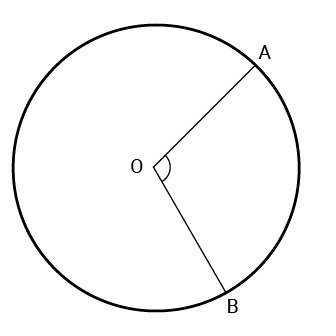
\includegraphics[width=0.75\linewidth]{images/cus19}
  \end{adjustbox}
\end{center}
\begin{choices}
  \CorrectChoice $\frac{7}{2}\pi$
  \choice $\frac{21}{2}\pi$
  \choice $12\pi$
  \choice $36\pi$
\end{choices}




\newpage




\question[1]
In the image shown, right triangle $LMN$ has a right angle at $M$. Altitude $PM$ is shown and $\angle NPM$ is a right angle. $LP=13$ and $PM=10$. Which of the following are closest to the length of $NP$?
\begin{center}
  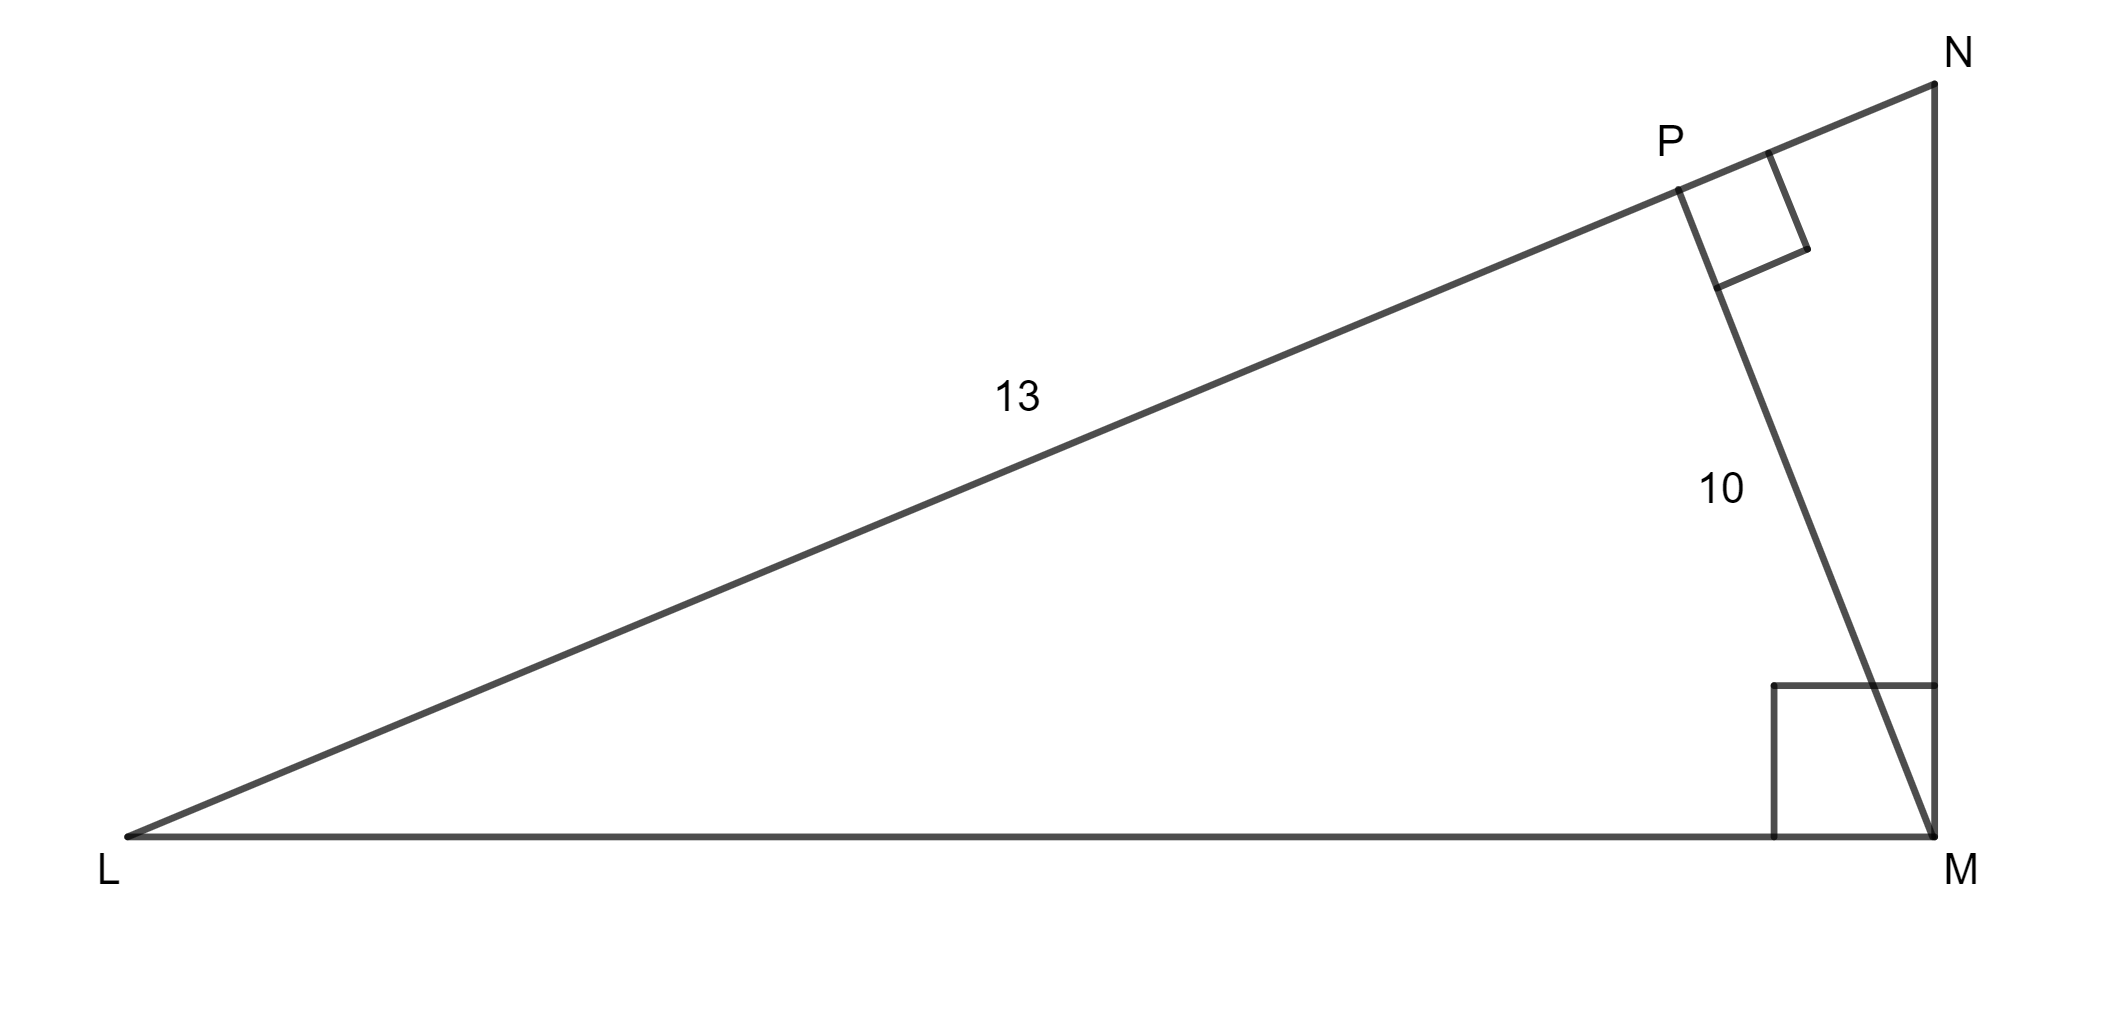
\includegraphics[width=0.90\linewidth]{images/cus20}
\end{center}
\begin{choices}
  \choice $3.0$
  \choice $6.2$
  \choice $7.1$
  \CorrectChoice $7.7$
\end{choices}

\question[1]
For the given function $f(x)=24x^2+bx+c$, $b$ and $c$ are constants, and the graph of $y=f(x)$ in the $xy$-plane passes through the points in the table below. What is the value of $b$?
\begin{center}
  \renewcommand{\arraystretch}{1.3}
  \setlength{\tabcolsep}{0.5em}
  \captionof{table}{$x$ and $f(x)$}\label{tab:sat-drill-10-f-quadratic}%
  \vspace{0.35em}
  \begin{adjustbox}{max width=\linewidth,clip=false,margin=0pt}
  \begin{tabular}{|c|c|}
    \hline
    \cellcolor[HTML]{E0E0E0}{$x$} & \cellcolor[HTML]{E0E0E0}{$f(x)$} \\
    \hline
    $-\frac{15}{8}$ & 0 \\
    \hline
    0 & $c$ \\
    \hline
    $\frac{11}{4}$ & 0 \\
    \hline
  \end{tabular}
  \end{adjustbox}
\end{center}
\begin{solution}
-21
\end{solution}



\newpage




\question[1]
Select values for the polynomial function $g(x)$ are shown in the table. Based on the values in the table, which of the following must be factors of $g(x)$?
\begin{center}
  \renewcommand{\arraystretch}{1.3}
  \setlength{\tabcolsep}{0.5em}
  \captionof{table}{$x$ and $g(x)$}\label{tab:sat-drill-10-g-sample}%
  \vspace{0.35em}
  \begin{adjustbox}{max width=\linewidth,clip=false,margin=0pt}
  \begin{tabular}{|c|c|}
    \hline
    \cellcolor[HTML]{E0E0E0}{$x$} & \cellcolor[HTML]{E0E0E0}{$g(x)$} \\
    \hline
    $-7$ & $10$ \\
    \hline
    $-4$ & $0$ \\
    \hline
    $0$ & $5$ \\
    \hline
    $3$ & $1$ \\
    \hline
    $5$ & $-6$ \\
    \hline
    $11$ & $0$ \\
    \hline
  \end{tabular}
  \end{adjustbox}
\end{center}
\begin{choices}
  \choice $(x-5)$
  \choice $(x+5)$
  \choice $(x-4)$ and $(x+11)$
  \CorrectChoice $(x+4)$ and $(x-11)$
\end{choices}

\question[1]
Some values of the linear function $f$ are shown in the table.
\begin{center}
  \renewcommand{\arraystretch}{1.3}
  \setlength{\tabcolsep}{0.5em}
  \captionof{table}{Linear $f$ values}\label{tab:sat-drill-10-f-linear}%
  \vspace{0.35em}
  \begin{adjustbox}{max width=\linewidth,clip=false,margin=0pt}
  \begin{tabular}{|c|c|c|c|c|}
    \hline
    \cellcolor[HTML]{E0E0E0}{$a$} & 3 & 6 & 9 & 12 \\
    \hline
    \cellcolor[HTML]{E0E0E0}{$f(a)$} & -2 & -1 & 0 & 1 \\
    \hline
  \end{tabular}
  \end{adjustbox}
\end{center}
Which of the following defines $f$?
\begin{choices}
  \CorrectChoice $f(a)=\frac{1}{3}a-3$
  \choice $f(a)=-\frac{1}{3}a-1$
  \choice $f(a)=a-5$
  \choice $f(a)=2a-8$
\end{choices}






\newpage




\question[1]
If $|7x+14|=98$ and $x$ is positive, what is the value of $x+2$?
\begin{solution}
14
\end{solution}

\question[1]
Stan's plant grows 2.5 inches per week. It is 15 inches tall now. In how many weeks will the plant be 42.5 inches tall?
\begin{solution}
11
\end{solution}

\question[1]
How many solutions does the given equation have?
\[
  3(x-2)-2(x-1)=-x+2(x+2)-8
\]
\begin{choices}
  \choice Zero
  \choice Exactly one
  \choice Exactly two
  \CorrectChoice Infinitely many
\end{choices}

\question[1]
For $f(x+3)=\sqrt{x^3}+17$, what is the value of $f(4)$?
\begin{choices}
  \CorrectChoice 18
  \choice 25
  \choice 28
  \choice 35.5
\end{choices}





\newpage



\question[1]
Theresa invested in a company, and the value of her investment increased by $9\%$ from 2021 to 2022. If the value of her investment in 2022 is $k$ times the value it was in 2021, what is the value of $k$?
\begin{choices}
  \choice 0.09
  \choice 0.9
  \CorrectChoice 1.09
  \choice 1.9
\end{choices}

\question[1]
Which of the following expressions can equal $-1$ for some value of $a$?
\begin{choices}
  \choice $|a-3|+2$
  \choice $|a-2|+1$
  \choice $|a-1|$
  \CorrectChoice $|a-2|-2$
\end{choices}

\question[1]
\[
  \begin{gathered}
  \frac{m}{n}=3 \\
  6(n-4)=m
  \end{gathered}
\]
The solution to the given system of equations is $(m, n)$. What is the value of $n$?
\begin{choices}
  \choice 4
  \CorrectChoice 8
  \choice 16
  \choice 24
\end{choices}





\newpage



\question[1]
In circle $O$, the length of $AO$ is 12 units and the length of minor arc $AB$ is $8\pi$. What is the measure, in degrees, of $\angle AOB$?
\begin{center}
  \begin{adjustbox}{max width=\linewidth,center}
    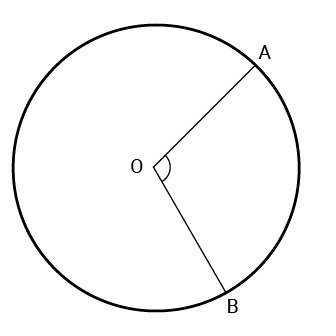
\includegraphics[width=0.55\linewidth]{images/cus21}
  \end{adjustbox}
\end{center}
\begin{solution}
120
\end{solution}

\question[1]
Which expression is equivalent to $\frac{x+4}{2x+2}+\frac{5}{x+1}$?
\begin{choices}
  \choice $\frac{x+7}{x+1}$
  \choice $\frac{x+9}{3x+3}$
  \CorrectChoice $\frac{x+14}{2x+2}$
  \choice $\frac{5x+20}{2x^2+4x+2}$
\end{choices}

\question[1]
Which of the following is the equation of $g(x)=2x$ when it is moved 1 unit to the left and 1 unit up?
\begin{choices}
  \choice $y=2x-1$
  \choice $y=2x+1$
  \CorrectChoice $y=2x+3$
  \choice $y=2x+5$
\end{choices}





\newpage



\question[1]
If $\overline{AB} \parallel \overline{DE}$, $AC=BC$, and the measure of $\angle ACB=88^\circ$, what is $m\angle FDE$?
\begin{center}
  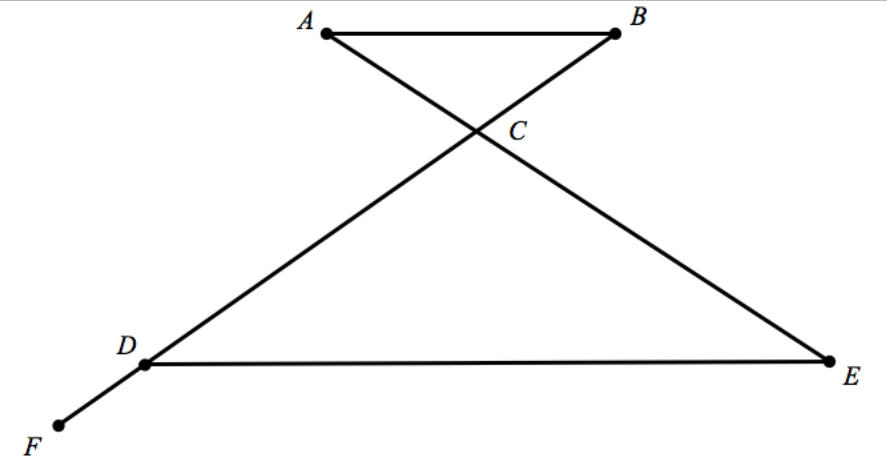
\includegraphics[width=0.90\linewidth]{images/cus22}
\end{center}
\begin{choices}
  \choice $88^\circ$
  \choice $92^\circ$
  \choice $128^\circ$
  \choice $134^\circ$
\end{choices}

\question[1]
The function $f(x)=mx+b$ and the function $g(x)=nx+b$ are defined for all real values of $x$. Which statement is true about the functions?
\begin{choices}
  \choice If $|m|>|n|$, then $f(x)>g(x)$ for all values of $x$.
  \choice If $|m|=|n|$, then $f(x)=g(x)$ for all values of $x$.
  \choice If $m>0$, then $f(x)>g(x)$ for all values of $x$.
  \CorrectChoice If $m\neq n$, then $f(x)=g(x)$ for only one value of $x$.
\end{choices}

\question[1]
Triangles $ABC$ and $BCD$ are right triangles, where $\angle A$ and $\angle D$ are right angles. If $AB=AC$ and $BD=CD$, what is the value of $\tan(\angle ABC)+\tan(\angle DBC)$?
\begin{solution}
2
\end{solution}





\newpage



\question[1]
The first term in a sequence is 21. Each term after the first term is 1.5 times the preceding term. If $s$ represents the $n$th term of the sequence, which equation gives $s$ in terms of $n$?
\begin{choices}
  \choice $s=1.5\left(21^n\right)$
  \choice $s=1.5\left(21^{n-1}\right)$
  \choice $s=21\left(1.5^n\right)$
  \CorrectChoice $s=21\left(1.5^{n-1}\right)$
\end{choices}

\question[1]
The distribution of test scores in Mrs. Keaton's English class is shown in the table.
\begin{center}
  \renewcommand{\arraystretch}{1.3}
  \setlength{\tabcolsep}{0.5em}
  \captionof{table}{Vocabulary scores}\label{tab:sat-drill-10-vocab}%
  \vspace{0.35em}
  \begin{adjustbox}{max width=\linewidth,clip=false,margin=0pt}
  \begin{tabular}{|l|l|}
    \hline
    \cellcolor[HTML]{E0E0E0}\textbf{Test Score} & \cellcolor[HTML]{E0E0E0}\textbf{Number of Students} \\
    \hline
    100 & 1 \\
    \hline
    90 & 5 \\
    \hline
    80 & 10 \\
    \hline
    70 & 8 \\
    \hline
    60 & 2 \\
    \hline
  \end{tabular}
  \end{adjustbox}
\end{center}
Which of the following sets of test scores, if added, would change the standard deviation of the distribution the least?
\begin{choices}
  \choice $60,60,60$
  \choice $60,100,100$
  \CorrectChoice $70,80,90$
  \choice $90,90,90$
\end{choices}

\question[1]
The graph of $2y-2x^2+14x=-36$ is translated to the left 3 units in the $xy$-plane. What is the positive $x$-coordinate of the $x$-intercept of the resulting graph?
\begin{solution}
6
\end{solution}

\question[1]
The graph of $y=f(x)$ is shown. Which of the following best represents the function $f(x)$?
\begin{center}
  \begin{adjustbox}{max width=\linewidth,center}
    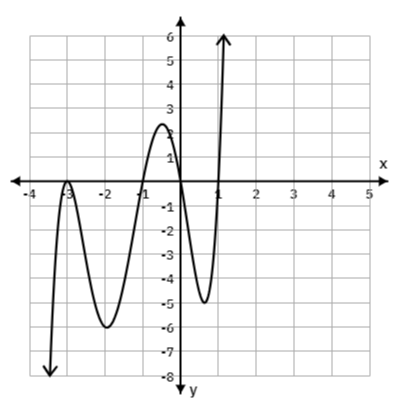
\includegraphics[width=0.75\linewidth]{images/cus23}
  \end{adjustbox}
\end{center}
\begin{choices}
  \choice $f(x)=x(x-1)(x+1)(x+3)^2$
  \choice $f(x)=x(x+1)(x-1)(x+3)$
  \choice $f(x)=(x-3)^2(x-1)(x+1)$
  \choice $f(x)=(x+3)^2(x+1)(x-1)$
\end{choices}

\question[1]
Which of the following expressions is equivalent to $\frac{x+3}{x^2-4x+3}+\frac{2}{x-1}$?
\begin{choices}
  \choice $\frac{1}{x-1}$
  \CorrectChoice $\frac{3}{x-3}$
  \choice $\frac{3x+3}{x^2-4x+3}$
  \choice $\frac{x+5}{x^2-3x+2}$
\end{choices}

\question[1]
If the given system of equations has no solution, what is the value of $ab$?
\[
  \begin{gathered}
  3x+by=36 \\
  ax-7y=24
  \end{gathered}
\]
\begin{solution}
-21
\end{solution}


\newpage



\question[1]
The point $(a,a)$ satisfies the linear inequality $y\leq mx+1$, and $a>0$. The value of $m$ must be greater than or equal to what value?
\begin{choices}
  \choice $\frac{1}{a}-1$
  \choice $a-1$
  \CorrectChoice $1-\frac{1}{a}$
  \choice $1-a$
\end{choices}

\question[1]
A ball is kicked off of a platform modeled by the equation $y=-5x^2+bx+10$, such that $y$ is height in feet, $x$ is seconds, and $b$ is a constant. The ball reaches a maximum height of 11.25 feet, and it takes 2 seconds to hit the ground. How many seconds does it take for the ball to reach its maximum height?
\begin{solution}
$\frac{1}{2}$
\end{solution}

\endgradingrange{sat-drill-10}
